\documentclass[a4paper,fleqn]{article}
\usepackage{graphics}
\title{Expopt version 2.2.a}
\author{Per-Olof Widmark}
\date{\today --- very tentative version}
\setcounter{secnumdepth}{0}
\let\headi=\subsection
\let\headii=\subsubsection
\def\file#1{{\sffamily\upshape\mdseries #1}}
\def\unix#1{{\ttfamily\upshape\mdseries #1}}
\def\kwd#1{{\mdseries\sffamily\slshape\mdseries #1}}
\def\kwditem[#1]{\item[\kwd{#1}]}
\begin{document}
\maketitle
%%==============================================================================
%% 1. Introduction
%%==============================================================================
\headi{1. Introduction}
This program is intended for optimizing primitive gaussian functions
for basis sets.

A primitive gaussian basis set is defined by a set of gaussian functions with
exponents $\{\alpha_k\}_{k=0,n-1}$ such that an atomic orbital will be expressed by
\begin{equation}
\varphi_p=\sum_{k=0}^{n-1} c_{k,p} r^\ell e^{-\alpha_k r^2}
\end{equation}
where $\ell$ is the orbital angular momentum.

The primitive exponents are updated according to
\begin{equation}
\ln\alpha_k = \ln\alpha_k^0 + \sum_{i=0}^{m-1} a_i g_i(k)
\end{equation}
where $\{\alpha_k^0\}_{k=0,n-1}$ is the start values for the exponents,
$\{g_i(k)\}_{i=0,m-1}$ is a set of generator functions and
$a_i$ is a set of coefficients to be determined.
The optimization criterion is the lowest possible energy.

There are a few different generators implemented described below in the
keywords section.
%%------------------------------------------------------------------------------
\headii{* How to use the program}
Expopt is basically an interpreter, when it reads a keyword then something
gets executed. For example if you have the keyword \kwd{Energy} in the input
the energy is computed with the basis set that is defined at that point, after
the completion of the energy calculation the next keyword is read.

Apart from an input file you need to supply an executable file with name \file{energy.ksh}.
Note that this file must be in the current directory. The purpose of this
executable is to produce an energy for a given primitive basis set.
\file{energy.ksh} reads the basis set from file \file{BASIS.DAT}
and writes a file \file{ENERGY.DAT} which contains a single number
namely the energy.

See page~\pageref{sec:energy.ksh} for an example of the file \file{energy.ksh}.
See page~\pageref{sec:basis.dat} for an example of the format of file \file{BASIS.DAT}.
See figure~\ref{fig:how_it_works} on page~\pageref{fig:how_it_works} for a graphical
description of how the program works.

\begin{figure}[htbp]
\begin{center}
\scalebox{0.50}{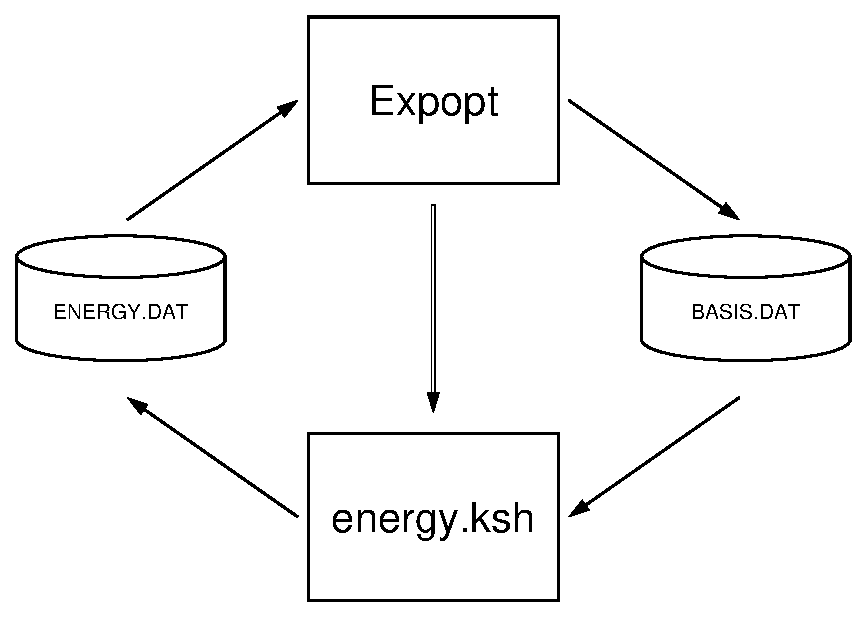
\includegraphics{fig}}
\end{center}
\caption{\label{fig:how_it_works}How expopt works}
\end{figure}
%%==============================================================================
%% 2. Keywords
%%==============================================================================
\headi{2. Keywords}
All keywords are case sensitive and are needed to be written as stated.
Use \verb+#+ at the start of a line for comments.
First line is a magic word:\\
\verb+#ExpOpt-2.0+
\begin{description}
\kwditem[ChangeZ] 
  Advanced keyword: Change Z value
\kwditem[Charge]
  Define the nuclear charge that is to be used in the calculation.
  Note that it is not automatically set the Z value when you define a shell
  and must be defined.
\kwditem[Define]
  Define the set of primitive exponents in a shell.
  On the following line(s) the atomic number, $\ell$-quantum number of the shell
  and the number of primitives are read, followed by reading all the exponents.
  Example:\\
  \verb+Define+\\
  \verb+7 0 6 100.0 30.0 9.0 2.7 0.81 0.243+\\
  defines an s-shell with 6 exponents for nitrogen (Z=7).
\kwditem[Energy]
  Calculate the energy for the shells currently defined.
\kwditem[Extend]
  Advanced keyword: two integers are required: a number of a shell, and for how much it should be extended. 
%\kwditem[Fit] Not implemented.
\kwditem[Generator]
  Select the generator for optimizing the basis sets.
  the generator can be one of
  \begin{description}
  \kwditem[HotTempered]
    Generator functions are:
      $g_0(k)=1$,
      $g_1(k)=k$,
      $g_2(k)=k^{-1}$,
      $g_3(k)=k^{-2}$,
      $g_4(k)=k^{-3}$ etc.
  \kwditem[HotPoly]
    Generator functions are:
      $g_0(k)=1$,
      $g_1(k)=k$,
      $g_2(k)=k^{-1}$,
      $g_3(k)=k^{2}$,
      $g_4(k)=k^{3}$ etc.
  \kwditem[Polynomial]
    Generator functions are: $g_i(k)=k^i$.
  \kwditem[Cosine]
    Generator functions are: $g_i(k)=\cos\left(\pi\frac{(k-1)*i}{n-1}\right)$, $i\in[0,n-1]$ and $k\in[1,n]$.
  \kwditem[Unit]
    Generator functions are: $g_i(k)=\delta_{i,k}$.
  \kwditem[SplitValence] %% first three terms as hottempered, then units from outside
    Generator functions are:
      $g_0(k)=1$,
      $g_1(k)=k$,
      $g_2(k)=k^{-1}$,
      $g_3(k)=\delta_{k,n-1}$,
      $g_4(k)=\delta_{k,n-2}$,
      $g_5(k)=\delta_{k,n-3}$ etc assuming that there are $n$ primitive functions.
  \kwditem[Exponential] Read the exponent value from the input
  \end{description}
\kwditem[gThreshold]
  Set the value for the norm of the gradient at convergence. Used with the QN method.
%\kwditem[Hessian] Not implemented.
%\kwditem[LineSearch] Not implemented.
\kwditem[Method]
  Select method for optimizing exponents.
  The method can be one of
  \begin{description}
  \kwditem[QN] Implemented, default.
  \kwditem[Amoeba] Implemented.
%  \kwditem[Auto] Not implemented.
  \kwditem[Powell] Powell (under development).
  \end{description}
\kwditem[Optimize]
  Optimize specified shell. Following the keyword is the number of the shell, 0 for s-shell, 1 for p-shell etc.
  Thereafter is a list of the directions along which the optimization is performed.
  For example\\
  \verb+Optimize 1 0 1 2+\\
  will optimize the p-shell in the space of the first three (0, 1, and 2) directions
  defined by the generator.
\kwditem[OptimizeWithDirections] 
\kwditem[Penalty] 
\kwditem[Print] 
%\kwditem[PrintDirections] Not implemented.
%\kwditem[Reorder] Not implemented.
\kwditem[SelectShell] 
\kwditem[PrintRaw] 
%\kwditem[Sort] Not implemented.
\kwditem[Step] 
\kwditem[Threshold] 
  Set the value for the difference in energy between two iterations at convergence.
  Used with the QN method.
\end{description}
%%==============================================================================
%% A. How the program works
%%==============================================================================
\headi{A. How the program works}
This is a short summary of how the program works.

The program itself have no capability to compute the energy for a given
primitive basis set but relies on an external code to do that.
The procedure is the following
\begin{enumerate}
\item Use the start exponents.
\item Create a file named \file{BASIS.DAT}.
\item Call an external program/script named \unix{energy.ksh} in the current directory.
\item Program/script \unix{energy.ksh} computes the energy using \file{BASIS.DAT}.
\item Program/script \unix{energy.ksh} computes and writes a file \file{ENERGY.DAT} that contains the energy.
\item The energy is read from file \file{ENERGY.DAT}.
\item If the optimization is converged, stop.
\item Decide on the next set of exponents to calculate an energy for and go to step 2.
\end{enumerate}
%%==============================================================================
%% B. Sample files
%%==============================================================================
\headi{B. Sample files}
In this appendix some sample files are listed.
%%------------------------------------------------------------------------------
\headii{* File \file{energy.ksh}}
\label{sec:energy.ksh}
This script is invoked by expopt and in turn starts a molcas job, waits until
completion and the extract the energies from the log file, and creates the
file \file{ENERGY.DAT}. In this particular case all RASSCF energies are
extracted and averaged. The first awk statement simply processes all lines
containing the string \texttt{Average CI energy} and prints the 4'th item (the energy)
and puts the results in a temporart file. The second awk statement then simply
averages these energies.

You could easily replace these awk commands with grep and sed combinations
that accomplish the same thing.
\begin{verbatim}
#!/bin/ksh
./Sn.energy.ksh > Sn.energy.log 2> Sn.energy.err
awk '/Average CI energy/{print $4}' Sn.energy.log > energy.tmp
awk -f average.awk energy.tmp > ENERGY.DAT
exit
\end{verbatim}
%%------------------------------------------------------------------------------
\headii{* File \file{average.awk}}
This is just an awk script that averages the energies in a file with multiple energies.
Could just as well have been inlined.
\begin{verbatim}
BEGIN{ s=0; n=0; }
{ s=s+$1; n=n+1; }
END{ s=s/n; printf(" %.10f\n",s); }
\end{verbatim}
%%------------------------------------------------------------------------------
\headii{* File \file{Sn.expopt.input}}
This is an input file for optimizing the s-shell for Sn atom.
\begin{verbatim}
#ExpOpt-2.0
#
# Optimizing Sn basis set
#
Threshold 0.10e-6
Charge 50.0
Generator HotTempered
#---
Define
 50 0 22  30478431.6 4625993.26 976417.834 248618.795 72736.2434 
          23688.1235 8402.61916 3188.63522 1274.98676 532.192307 
          229.810408 98.2017082 44.8412729 20.8208529 9.74349605 
          4.53424229 2.02629829 0.84940458 0.32027879 0.10083040
          0.04033216 0.01613286 
Define
 50 1 19  1224643.53 177456.003 37958.6836 10372.4236 3414.51095 
          1289.09077 537.195567 240.599182 113.302609 55.3080046 
          27.3028315 13.4581595 6.74330142 3.13136544 1.46412063 
          0.65369320 0.18811129 0.06053112 0.02421245
Define
 50 2 13  1274.98676 532.192307 229.810408 98.2017082 44.8412729 
          20.8208529 9.74349605 4.53424229 2.02629829 0.84940458 
          0.32027879 0.12811152 0.05124461
#---
#Energy
Optimize 0 0 1
#Optimize 1 0 1
#Optimize 2 0 1
\end{verbatim}
%%------------------------------------------------------------------------------
\headii{* File \file{ENERGY.DAT}}
This file should contain only one single floating point number representing the
energy.
\begin{verbatim}
 -6172.3175324500
\end{verbatim}
%%------------------------------------------------------------------------------
\headii{* File \file{BASIS.DAT}}
\label{sec:basis.dat}
The file \file{BASIS.DAT} is in a format suitable for SEWARD. The first line
contains the nuclear charge and the highest angular momentum.
Then for each $\ell$-shell you have:
one line with two integers, one for the number of primitives and one for the
number of contractions files. This is followed by all the exponents
and finally the contraction matrix which is simply the unit matrix.
\begin{verbatim}
 50.00 2
 22 22
30478431.60000000
4625993.26000000
976417.83400000
248618.79500000
72736.24340000
23688.12350000
8402.61916000
3188.63522000
1274.98676000
532.19230700
229.81040800
98.20170820
44.84127290
20.82085290
9.74349605
4.53424229
2.02629829
0.84940458
0.32027879
0.10083040
0.04033216
0.01613286
1. 0. 0. 0. 0. 0. 0. 0. 0. 0. 0. 0. 0. 0. 0. 0. 0. 0. 0. 0. 0. 0. 
0. 1. 0. 0. 0. 0. 0. 0. 0. 0. 0. 0. 0. 0. 0. 0. 0. 0. 0. 0. 0. 0. 
0. 0. 1. 0. 0. 0. 0. 0. 0. 0. 0. 0. 0. 0. 0. 0. 0. 0. 0. 0. 0. 0. 
0. 0. 0. 1. 0. 0. 0. 0. 0. 0. 0. 0. 0. 0. 0. 0. 0. 0. 0. 0. 0. 0. 
0. 0. 0. 0. 1. 0. 0. 0. 0. 0. 0. 0. 0. 0. 0. 0. 0. 0. 0. 0. 0. 0. 
0. 0. 0. 0. 0. 1. 0. 0. 0. 0. 0. 0. 0. 0. 0. 0. 0. 0. 0. 0. 0. 0. 
0. 0. 0. 0. 0. 0. 1. 0. 0. 0. 0. 0. 0. 0. 0. 0. 0. 0. 0. 0. 0. 0. 
0. 0. 0. 0. 0. 0. 0. 1. 0. 0. 0. 0. 0. 0. 0. 0. 0. 0. 0. 0. 0. 0. 
0. 0. 0. 0. 0. 0. 0. 0. 1. 0. 0. 0. 0. 0. 0. 0. 0. 0. 0. 0. 0. 0. 
0. 0. 0. 0. 0. 0. 0. 0. 0. 1. 0. 0. 0. 0. 0. 0. 0. 0. 0. 0. 0. 0. 
0. 0. 0. 0. 0. 0. 0. 0. 0. 0. 1. 0. 0. 0. 0. 0. 0. 0. 0. 0. 0. 0. 
0. 0. 0. 0. 0. 0. 0. 0. 0. 0. 0. 1. 0. 0. 0. 0. 0. 0. 0. 0. 0. 0. 
0. 0. 0. 0. 0. 0. 0. 0. 0. 0. 0. 0. 1. 0. 0. 0. 0. 0. 0. 0. 0. 0. 
0. 0. 0. 0. 0. 0. 0. 0. 0. 0. 0. 0. 0. 1. 0. 0. 0. 0. 0. 0. 0. 0. 
0. 0. 0. 0. 0. 0. 0. 0. 0. 0. 0. 0. 0. 0. 1. 0. 0. 0. 0. 0. 0. 0. 
0. 0. 0. 0. 0. 0. 0. 0. 0. 0. 0. 0. 0. 0. 0. 1. 0. 0. 0. 0. 0. 0. 
0. 0. 0. 0. 0. 0. 0. 0. 0. 0. 0. 0. 0. 0. 0. 0. 1. 0. 0. 0. 0. 0. 
0. 0. 0. 0. 0. 0. 0. 0. 0. 0. 0. 0. 0. 0. 0. 0. 0. 1. 0. 0. 0. 0. 
0. 0. 0. 0. 0. 0. 0. 0. 0. 0. 0. 0. 0. 0. 0. 0. 0. 0. 1. 0. 0. 0. 
0. 0. 0. 0. 0. 0. 0. 0. 0. 0. 0. 0. 0. 0. 0. 0. 0. 0. 0. 1. 0. 0. 
0. 0. 0. 0. 0. 0. 0. 0. 0. 0. 0. 0. 0. 0. 0. 0. 0. 0. 0. 0. 1. 0. 
0. 0. 0. 0. 0. 0. 0. 0. 0. 0. 0. 0. 0. 0. 0. 0. 0. 0. 0. 0. 0. 1. 
 19 19
1224643.53000000
177456.00300000
37958.68360000
10372.42360000
3414.51095000
1289.09077000
537.19556700
240.59918200
113.30260900
55.30800460
27.30283150
13.45815950
6.74330142
3.13136544
1.46412063
0.65369320
0.18811129
0.06053112
0.02421245
1. 0. 0. 0. 0. 0. 0. 0. 0. 0. 0. 0. 0. 0. 0. 0. 0. 0. 0. 
0. 1. 0. 0. 0. 0. 0. 0. 0. 0. 0. 0. 0. 0. 0. 0. 0. 0. 0. 
0. 0. 1. 0. 0. 0. 0. 0. 0. 0. 0. 0. 0. 0. 0. 0. 0. 0. 0. 
0. 0. 0. 1. 0. 0. 0. 0. 0. 0. 0. 0. 0. 0. 0. 0. 0. 0. 0. 
0. 0. 0. 0. 1. 0. 0. 0. 0. 0. 0. 0. 0. 0. 0. 0. 0. 0. 0. 
0. 0. 0. 0. 0. 1. 0. 0. 0. 0. 0. 0. 0. 0. 0. 0. 0. 0. 0. 
0. 0. 0. 0. 0. 0. 1. 0. 0. 0. 0. 0. 0. 0. 0. 0. 0. 0. 0. 
0. 0. 0. 0. 0. 0. 0. 1. 0. 0. 0. 0. 0. 0. 0. 0. 0. 0. 0. 
0. 0. 0. 0. 0. 0. 0. 0. 1. 0. 0. 0. 0. 0. 0. 0. 0. 0. 0. 
0. 0. 0. 0. 0. 0. 0. 0. 0. 1. 0. 0. 0. 0. 0. 0. 0. 0. 0. 
0. 0. 0. 0. 0. 0. 0. 0. 0. 0. 1. 0. 0. 0. 0. 0. 0. 0. 0. 
0. 0. 0. 0. 0. 0. 0. 0. 0. 0. 0. 1. 0. 0. 0. 0. 0. 0. 0. 
0. 0. 0. 0. 0. 0. 0. 0. 0. 0. 0. 0. 1. 0. 0. 0. 0. 0. 0. 
0. 0. 0. 0. 0. 0. 0. 0. 0. 0. 0. 0. 0. 1. 0. 0. 0. 0. 0. 
0. 0. 0. 0. 0. 0. 0. 0. 0. 0. 0. 0. 0. 0. 1. 0. 0. 0. 0. 
0. 0. 0. 0. 0. 0. 0. 0. 0. 0. 0. 0. 0. 0. 0. 1. 0. 0. 0. 
0. 0. 0. 0. 0. 0. 0. 0. 0. 0. 0. 0. 0. 0. 0. 0. 1. 0. 0. 
0. 0. 0. 0. 0. 0. 0. 0. 0. 0. 0. 0. 0. 0. 0. 0. 0. 1. 0. 
0. 0. 0. 0. 0. 0. 0. 0. 0. 0. 0. 0. 0. 0. 0. 0. 0. 0. 1. 
 13 13
1274.98676000
532.19230700
229.81040800
98.20170820
44.84127290
20.82085290
9.74349605
4.53424229
2.02629829
0.84940458
0.32027879
0.12811152
0.05124461
1. 0. 0. 0. 0. 0. 0. 0. 0. 0. 0. 0. 0. 
0. 1. 0. 0. 0. 0. 0. 0. 0. 0. 0. 0. 0. 
0. 0. 1. 0. 0. 0. 0. 0. 0. 0. 0. 0. 0. 
0. 0. 0. 1. 0. 0. 0. 0. 0. 0. 0. 0. 0. 
0. 0. 0. 0. 1. 0. 0. 0. 0. 0. 0. 0. 0. 
0. 0. 0. 0. 0. 1. 0. 0. 0. 0. 0. 0. 0. 
0. 0. 0. 0. 0. 0. 1. 0. 0. 0. 0. 0. 0. 
0. 0. 0. 0. 0. 0. 0. 1. 0. 0. 0. 0. 0. 
0. 0. 0. 0. 0. 0. 0. 0. 1. 0. 0. 0. 0. 
0. 0. 0. 0. 0. 0. 0. 0. 0. 1. 0. 0. 0. 
0. 0. 0. 0. 0. 0. 0. 0. 0. 0. 1. 0. 0. 
0. 0. 0. 0. 0. 0. 0. 0. 0. 0. 0. 1. 0. 
0. 0. 0. 0. 0. 0. 0. 0. 0. 0. 0. 0. 1. 
\end{verbatim}
%%============================================================================
%% Done
%%==============================================================================
\end{document}
